\section{Benutzeroberfläche}
\label{sec:Benutzeroberfläche}


Dieser Abschnitt beschäftigt sich mit der grundlegenden Gestaltung der Benutzeroberfläche für die unterschiedlichen Nutzer. Zunächst


\begin{tabular}{p{1.5cm}p{14.5cm}}
 /B10/	& Fensterlayout, Dialogstruktur und Mausbedienung entsprechen dem Windows-Gestaltungs-Regelwerk. \\[0.25cm]	 
\end{tabular}

\begin{tabular}{p{1.5cm}p{14.5cm}}
 /B11/	& Sämtliche Daten sind passwortgeschützt und dürfen nur von autorisierten Mitarbeitern des Lehrstuhls bearbeitet werden. \\[0.25cm]	 
\end{tabular}


\subsection{Bildschirmlayout}

\begin{tabular}{p{1.5cm}p{14.5cm}}
 /B20/	& Übersichtliche Gestaltung der Funktionen und intuitive Nutzung durch ein angepasstes Bildschirmlayout. \\[0.25cm]	 
\end{tabular}

\begin{tabular}{p{1.5cm}p{14.5cm}}
 /B30/	& Standardmäßig startet das Programm mit einer Suchmaske. Weitere Funktionen sind via Tabs und einer Anmeldung erreichbar. \\[0.25cm]	 
\end{tabular}

\begin{tabular}{p{1.5cm}p{14.5cm}}
 /BF40/	& Individuelle Anpassungsfähigkeit des Bildschirmlayouts an die Fenstergröße sollte möglich sein. \\[0.25cm]	 
\end{tabular}

\subsection{Drucklayout}

\begin{tabular}{p{1.5cm}p{14.5cm}}
 /B50/	& Nicht Angemeldete Nutzer können über die Auswahl verschiedener Lehrveranstaltungen einen Stundenplan im PDF-Format in Din-A4 Größe erzeugen lassen. \\[0.25cm]	 
\end{tabular}

\begin{tabular}{p{1.5cm}p{14.5cm}}
 /B60/	& Die Hausverwaltungsnutzer können folgende Raumpläne im PFD-Format und Din-A4 Größe erzeugen lassen. \\[0.25cm]	 
\end{tabular}

\begin{tabular}{p{1.5cm}p{14.5cm}}
 /B70/	& Mitarbeiter der Lehrstühle können personen- oder lehrstuhlbezogene Wochenpläne in ein PDF-Format exportieren in Din-A4 Größe. \\[0.25cm]	 
\end{tabular}
 
\subsection{Tastaturbelegung}

\begin{tabular}{p{1.5cm}p{14.5cm}}
 /B80/	& Die Bedienoberfläche ist auf eine Bedienung mittels Tastatur und Maus auszulegen. Benutzer in der Studentenrolle können keine Eingaben mittels der Tastatur vornehmen. Dozenten und die Hausverwaltung brauchen die Tastatur um verschiedene Funktionen auszuführen. \\[0.25cm]	 
\end{tabular}

\begin{tabular}{p{1.5cm}p{14.5cm}}
 /BF81/	& Mögliche individuelle, nicht dem Windows Standard entsprechende, Tastaturbelegungen sind ein mögliches  Wunschkriterium. \\[0.25cm]	 
\end{tabular}


\subsection{Dialogstruktur}

\begin{tabular}{p{1.5cm}p{14.5cm}}
 /B90/	& Zu Beachten ist: ISO 9241-10: 1996 bzgl. der ergonomischen Anforderungen für Bürotätigkeiten mit Bildschirmgeräten, Teil 10: Grundsätze der Dialoggestaltung. \\[0.25cm]	 
\end{tabular}

\begin{tabular}{p{1.5cm}p{14.5cm}}
 /B91/	& Folgende Rollen sind zu unterscheiden: \\[0.25cm]	 
\end{tabular}\\


\begin{table}[h]
\begin{tabular}{l|l}
Rolle&Rechte\\
\hline
\hline
Student & (F01), F60 , FW61, F130 \\
\hline
Dozent & F01, F20, FW21, F30, F70, F140, F150  \\
\hline
Verwaltungsangestellter & F01, F10, FW21, F40, F50, F51, F80, F90,  \\
\hline
Alle & F01, F100, F110, F120
\end{tabular}
\end{table}

Nachfolgend wird die Dialogstruktur durch den GUI (General User Interface) Prototypen verdeutlicht um die Benutzeroberfläche vorzustellen und zu erläutern.\\
\begin{figure}
\begin{center}
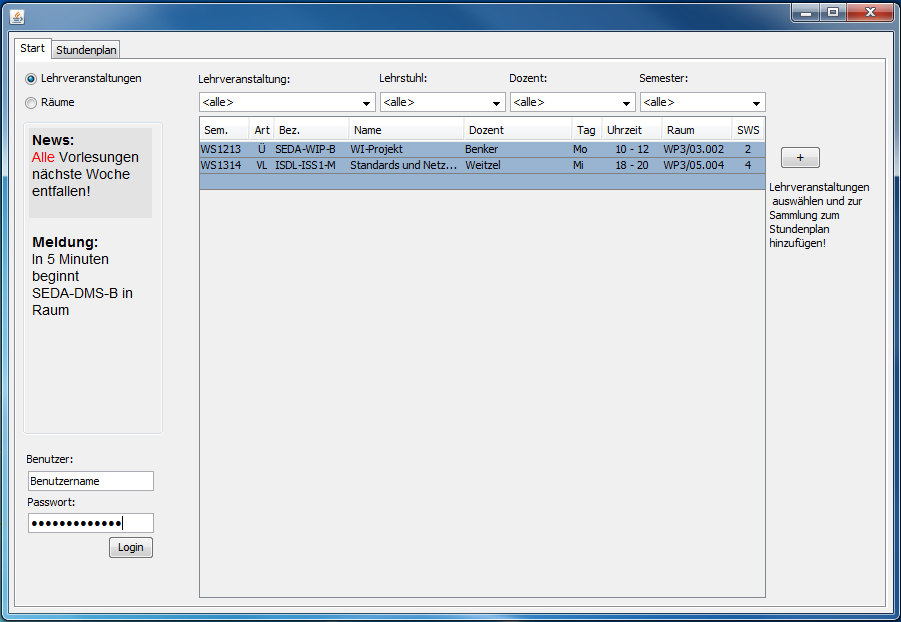
\includegraphics{../images/section_7/HauptseiteAlle.PNG}
\caption{GUI Startseite, rollenunabhängig}
\label{img:hauptseite}
\end{center}
\end{figure}